\documentclass[11pt]{article}

% ============================================================
% Packages
% ============================================================
\usepackage[utf8]{inputenc}
\usepackage[margin=1in]{geometry}
\usepackage{amsmath,amssymb,amsthm}
\usepackage{graphicx}
\usepackage{booktabs}
\usepackage{xcolor}
\usepackage{hyperref}
\usepackage{tikz}
\usepackage{enumitem}
\usepackage{pgfplots}

\pgfplotsset{compat=1.18}

% ============================================================
% Document Formatting
% ============================================================
\setlength{\parskip}{0.6em}
\setlength{\parindent}{0pt}

% ============================================================
% List Formatting
% ============================================================
\setlist[enumerate]{
    leftmargin=2em,
    itemsep=0.25em
}

% ============================================================
% Solution Environment
% ============================================================
\newenvironment{solution}
    {\par\noindent\textbf{Solution.}\par}
    {\par}

% ============================================================
% Link Styling
% ============================================================
\hypersetup{
    colorlinks=true,
    linkcolor=blue,
    urlcolor=cyan
}

% ============================================================
% Metadata
% ============================================================
\title{Ordinary Differential Equations}
\author{Chris Ritter}
\date{August 18, 2026}

% ============================================================
% Document
% ============================================================

\begin{document}

\maketitle
\tableofcontents
\newpage

\section{Introduction to Ordinary Differential Equations}
Differential equations are mathematical equations that relate a function with its derivatives. In physical applications, the independent variable often represents time ($t$) or space ($x$), and the dependent variable represents a changing quantity ($y$ or $v$).

Here are a few introductory examples of explicit functions and the differential equations they satisfy:
\[
  y = x^2 \implies \frac{dy}{dx} = 2x = f(x)
\]
\[
  y = e^x \implies \frac{dy}{dx} = y = f(y)
\]
\[
  x^2 + y^2 = R^2 \implies \frac{dy}{dx} = -\frac{x}{y} = f(x,y)
\]

In general, a first-order ordinary differential equation (ODE) can be written in the form:
\[
  \frac{dy}{dx} = h(x,y) \quad \text{or} \quad \frac{dy}{dt} = h(t,y)
\]

---

\section{Falling Object Model}
Consider an object of mass $m$ falling through the atmosphere near the Earth's surface. We model the forces acting on the object to understand its velocity $v(t)$ over time.

\subsection{Physical Modeling and Forces}
There are two primary forces acting on the object: gravity pulling it downward and air resistance (drag) opposing the motion upward.

\begin{center}
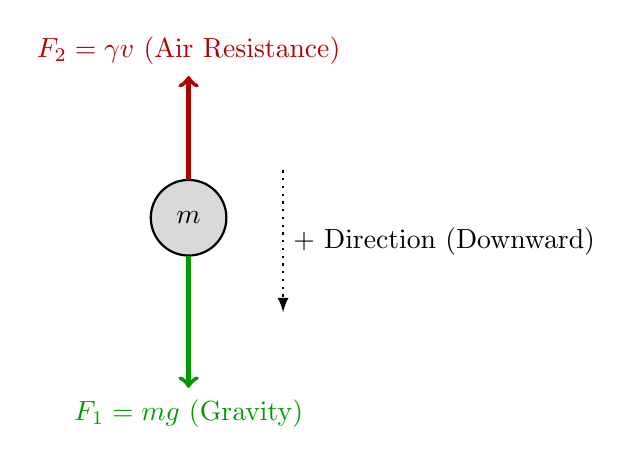
\begin{tikzpicture}[scale=1.2]
    % Draw the falling object (ball)
    \draw[fill=gray!30, thick] (0,0) circle (0.4cm) node {$m$};
    
    % Gravity Force Arrow (Fixed color here to prevent crash)
    \draw[->, green!60!black, ultra thick] (0,-0.4) -- (0,-1.8) node[below] {$F_1 = mg$ (Gravity)};
    
    % Drag Force Arrow
    \draw[->, red!70!black, ultra thick] (0,0.4) -- (0,1.5) node[above] {$F_2 = \gamma v$ (Air Resistance)};
    
    % Direction indicator
    \draw[-latex, dotted, thick] (1,0.5) -- (1,-1) node[midway, right] {$+$ Direction (Downward)};
\end{tikzpicture}
\end{center}

Where:
\begin{itemize}
    \item $m$, $g$, and $\gamma$ are positive constant parameters.
    \item $g = 9.81 \text{ m/sec}^2$ represents acceleration due to gravity.
    \item $\gamma$ represents the drag coefficient (resistance parameter).
\end{itemize}

Applying Newton's Second Law ($F = ma$):
\[
  ma = F_1 - F_2
\]
Since velocity is $v = v(t)$ and acceleration is $a = a(t) = \frac{dv}{dt}$, we can substitute these into the force balance:
\[
  m \frac{dv}{dt} = mg - \gamma v
\]
Dividing through by the mass $m$ yields our explicit first-order linear ODE for velocity:
\[
  \frac{dv}{dt} = g - \frac{\gamma}{m}v
\]

\subsection{Numerical Example \& Direction Field Analysis}
Let us assign specific numbers to the parameters:
\begin{itemize}
    \item Mass $m = 10 \text{ kg}$
    \item Drag coefficient $\gamma = 2 \text{ kg/sec}$
    \item Acceleration due to gravity $g = 9.8 \text{ m/sec}^2$
\end{itemize}

The equation becomes:
\[
  \frac{dv}{dt} = 9.8 - \frac{v}{5}
\]
Assuming the object is dropped from rest, we have the initial condition: $v(0) = 0$.

By evaluating the derivative $\frac{dv}{dt}$ at various values of $v$, we can track how the slope of our solution changes:
\begin{itemize}
    \item If $v = 0 \implies \frac{dv}{dt} = 9.8$
    \item If $v = 10 \implies \frac{dv}{dt} = 7.8$
    \item If $v = 40 \implies \frac{dv}{dt} = 1.8$
    \item If $v = 49 \implies \frac{dv}{dt} = 0$
    \item If $v = 60 \implies \frac{dv}{dt} = -2.2$
    \item If $v = 80 \implies \frac{dv}{dt} = -6.2$
\end{itemize}

Visualizing these slopes creates a **direction field** (or slope field). Below is a sketch of the direction field along with the equilibrium solutions:

\begin{center}
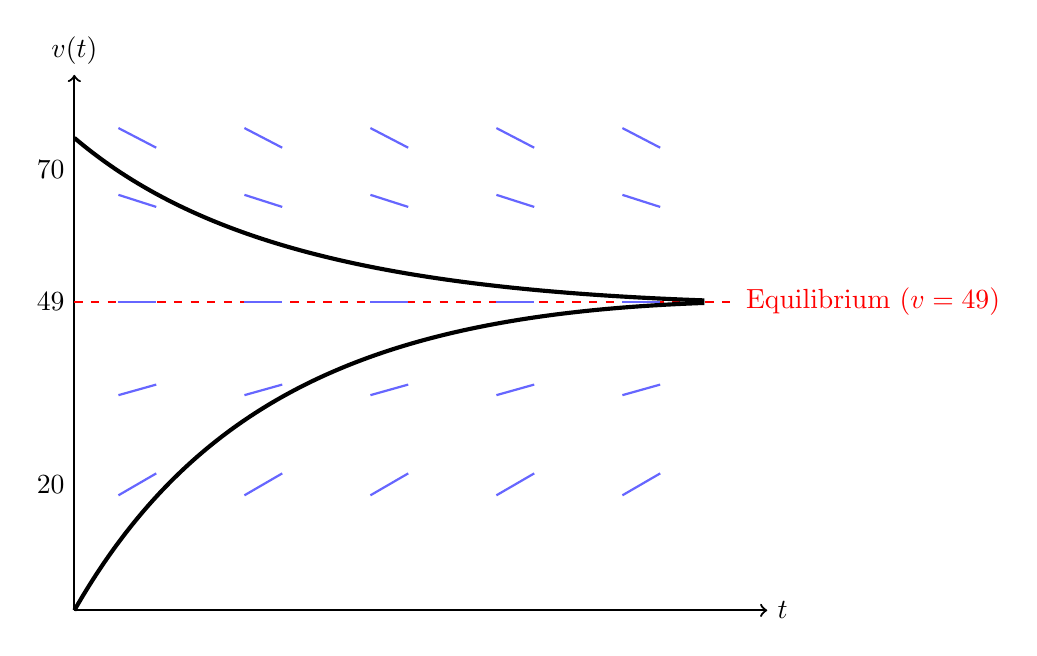
\begin{tikzpicture}[scale=0.08]
    % Axes
    \draw[->, thick] (0,0) -- (110,0) node[right] {$t$};
    \draw[->, thick] (0,0) -- (0,85) node[above] {$v(t)$};
    
    % Labels on v-axis
    \node[left] at (0,49) {$49$};
    \node[left] at (0,20) {$20$};
    \node[left] at (0,70) {$70$};
    
    % Equilibrium line
    \draw[dashed, red, thick] (0,49) -- (105,49) node[right] {Equilibrium ($v=49$)};
    
    % Generate slope field segments programmatically
    \foreach \t in {10, 30, 50, 70, 90} {
        % For v = 20 (Slope = 5.8)
        \draw[blue!60, thick] (\t-3, 20-1.74) -- (\t+3, 20+1.74);
        % For v = 35 (Slope = 2.8)
        \draw[blue!60, thick] (\t-3, 35-0.84) -- (\t+3, 35+0.84);
        % For v = 49 (Slope = 0)
        \draw[blue!60, thick] (\t-3, 49) -- (\t+3, 49);
        % For v = 65 (Slope = -3.2)
        \draw[blue!60, thick] (\t-3, 65+0.96) -- (\t+3, 65-0.96);
        % For v = 75 (Slope = -5.2)
        \draw[blue!60, thick] (\t-3, 75+1.56) -- (\t+3, 75-1.56);
    }
    
    % Sample trajectories
    \draw[line width=1.5pt, black] (0,0) .. controls (20,35) and (50,47) .. (100,48.8);
    \draw[line width=1.5pt, black] (0,75) .. controls (20,58) and (50,51) .. (100,49.2);
\end{tikzpicture}
\end{center}

\subsection{Qualitative Behavior Conclusions}
From this directional analysis, we observe that as $t \to \infty$, the velocity $v(t) \to 49 \text{ m/sec}$. 
\begin{enumerate}
    \item If $v(0) = 49$, then $v(t) = 49$ for all $t$ (constant solution).
    \item If $v(0) < 49$, then $v(t) \to 49$ as $t \to \infty$ in a strictly increasing fashion.
    \item If $v(0) > 49$, then $v(t) \to 49$ as $t \to \infty$ in a strictly decreasing fashion.
\end{enumerate}

\subsection{General Algebraic Conclusions}
Returning to the algebraic equation $\frac{dv}{dt} = g - \frac{\gamma}{m}v$, setting $\frac{dv}{dt} = 0$ yields the **equilibrium velocity** (also known as the limiting or terminal velocity):
\[
  v_e = \frac{mg}{\gamma}
\]
\begin{enumerate}
    \item If $v(0) < \frac{mg}{\gamma}$, then $v(t) \to \frac{mg}{\gamma}$ as $t \to \infty$ in an increasing way.
    \item If $v(0) > \frac{mg}{\gamma}$, then $v(t) \to \frac{mg}{\gamma}$ as $t \to \infty$ in a decreasing way.
    \item If $v(0) = \frac{mg}{\gamma}$, then $v(t) = \frac{mg}{\gamma}$ is a constant equilibrium solution.
\end{enumerate}

---

\section{Population Model}
Let $p(t)$ represent the population size of field mice at time $t$. 

\subsection{Scenario A: Exponential Growth (No Predation)}
Assuming ideal environmental conditions with no predators, the population grows at a rate directly proportional to its current size:
\[
  \frac{dp}{dt} = rp
\]
Where $r > 0$ represents the constant intrinsic growth rate parameter.

\subsection{Scenario B: Introducing Predation (Owls)}
Now assume a population of owls relocates to the area and kills/eats a steady number of mice, $k$, per unit of time. The rate equation shifts to account for this constant loss:
\[
  \frac{dp}{dt} = rp - k
\]

\subsection{Quantitative Analysis and Slopes}
Let's analyze a specific case where the intrinsic growth rate $r = \frac{1}{2}$ and the predation rate $k = 450$ mice/month. Our differential equation becomes:
\[
  \frac{dp}{dt} = \frac{1}{2}p - 450
\]

To evaluate the long-term behavior of the mouse population, we find the equilibrium point by setting $\frac{dp}{dt} = 0$:
\[
  \frac{1}{2}p - 450 = 0 \implies p_e = \frac{k}{r} = \frac{450}{1/2} = 900 \text{ mice}
\]

\textbf{Long-Term Dynamic Behaviors:}
\begin{itemize}
    \item \textbf{Thriving Population ($p(0) > \frac{k}{r}$):} If the starting population is greater than 900, the reproductive rate outpaces predation. The growth rate $\frac{dp}{dt}$ stays positive and expands, meaning $p(t) \to \infty$ as $t \to \infty$.
    \item \textbf{Extinction Event ($p(0) < \frac{k}{r}$):} If the starting population is fewer than 900, the owls consume mice faster than they can reproduce. The growth rate $\frac{dp}{dt}$ is negative, meaning $p(t) \to 0$ in finite time (mathematically heading towards $-\infty$).
    \item \textbf{Perfect Balance ($p(0) = \frac{k}{r}$):} If the starting population is exactly 900, the birth rate perfectly counters the predation rate. The population remains static at $p(t) = 900$.
\end{itemize}

\end{document}
